% !TeX encoding = UTF-8
% !TeX program = pdflatex
% !BIB program = biber

\documentclass[
        english,biblatex
    ]{lni}

\addbibresource{my-paper.bib}


% Standard packages
\usepackage{graphicx}
\usepackage{longtable}
\usepackage{booktabs}
\usepackage{array}
\usepackage{multirow}
\usepackage{wrapfig}
\usepackage{float}
\usepackage{colortbl}
\usepackage{pdflscape}
\usepackage{tabularx}
\usepackage{threeparttable}
\usepackage{threeparttablex}
\usepackage[normalem]{ulem}
\usepackage{makecell}
\usepackage{multicol}


\usepackage{framed} % Needed for code blocks


% solve \tightlist error
\providecommand{\tightlist}{%
    \setlength{\itemsep}{0pt}\setlength{\parskip}{0pt}}

% solve \pandocbounded error
\providecommand{\pandocbounded}[1]{#1}



\begin{document}

% Title
        \title[]{Preliminary Comparison of RSE and DS Competences}
    
    
    


\author[1]{Julian Dehne}{julian.dehne@gi.de}{0000-0001-9265-9619}
\author[2]{Jan Philipp Thiele}{jan-philipp.thiele@tu-braunschweig.de}{0000-0002-8901-6660}
\author[3]{Jeremy Cohen}{jeremy.cohen@imperial.ac.uk}{0000-0003-4312-2537}
\author[4]{Katrin Schöning-Stierand}{\href{mailto:katrin.schoening-stierand@uni-hamburg.de}{katrin.schoening-stierand@uni-hamburg.de}}{0000-0003-3248-8023}
\author[5]{Florian Goth}{\href{mailto:Florian.Goth@uni-wuerzburg.de}{Florian.Goth@uni-uerzburg.de}}{0000-0003-2707-4790}
\author[6]{Jan Linxweiler}{\href{mailto:j.linxweiler@tu-braunschweig.de}{j.linxweiler@tu-braunschweig.de}}{0000-0002-2755-5087}
\author[7]{Anna-Lena Lamprecht}{\href{mailto:anna-lena.lamprecht@uni-potsdam.de}{anna-lena.lamprecht@uni-potsdam.de}}{0000-0003-1953-5606}

\affil[1]{Gesellschaft für Informatik\\Bildung und Gesellschaft\\
Weydingerstraße 14-16\\10178 Berlin\\Deutschland}
\affil[2]{TU Braunschweig\\Universitätsbibliothek\\
Universitätspl. 1, 38106 Braunschweig\\Deutschland}
\affil[3]{University 3\\Department\\Address\\Country}
\affil[4]{Universität Hamburg\\Hub of Computing and Data Science\\Albert-Einstein-Ring 8\\22761 Hamburg\\Deutschland}
\affil[5]{Universität Würzburg\\Institut für theoretische Physik 1\\Am Hubland\\97070 Würzburg\\Deutschland}
\affil[6]{TU Braunschweig\\Universitätsbibliothek\\
Universitätspl. 1, 38106 Braunschweig\\Deutschland}
\affil[7]{Universität Potsdam\\Chair of Software Engineering\\An der Bahn 2\\14476 Potsdam\\Deutschland}


    \maketitle

% Abstract
        \begin{abstract}
        Die LaTeX-Klasse \texttt{lni} setzt die Layout-Vorgaben für
        Beiträge in LNI Konferenzbänden um. Dieses Dokument beschreibt
        ihre Verwendung und ist ein Beispiel für die entsprechende
        Darstellung.
    \end{abstract}
    
% Keywords
        \begin{keywords}
        Research Software-Engineering \and Data Science \and Competences
    \end{keywords}
    
% Body
    \section{Introduction}\label{introduction}

    Computers and software have become vital elements of the research
    process across almost all domains. They enable researchers to
    collect and process ever-increasing amounts of data, simulate a wide
    range of phenomena on previously unexplored scales, and discover
    previously inconceivably complex structures in nature and societies
    via machine learning (ML). This importance of computation and
    digitally-aided data analysis in research means that digital skills
    are now required by researchers at all career levels. However, as
    there are more digital skills than an individual reseracher can
    master to perfection, there is an increasing demand for specialized
    support personnel that interfaces between researchers and their
    digtial tools, and provides targeted help and additional expertise
    when needed. Below we introduce some of usch roles that have emerged
    in the research landscape (roughly in the order in which the terms
    started appearing).

    \begin{itemize}
    \item
      \textbf{Research data managers} (also aka data stewards) are
      responsible for overseeing the lifecycle of research data, from
      its creation and collection to its storage, sharing, and
      preservation \cite{https://doi.org/10.5281/zenodo.4915861}. They
      are responsible for organizing, storing, and maintaining the
      integrity of data collected during research projects. They develop
      and implement data management plans, ensuring data is accurate,
      secure, and compliant with legal and ethical standards in order to
      improve the handling of research data at every point in the data
      cycle (FIXME: Insert picture of data cycle). They work closely
      with researchers to support data collection, cleaning,
      documentation, and sharing. Additionally, research data managers
      often facilitate data archiving and ensure that data is accessible
      for future use or replication. Within Germany, numerous regional
      networks have been formed. More information can be found at
      \cite{fdminfo}.
    \item
      \textbf{Data scientists} are professionals who combine expertise
      in programming, statistics, machine learning, and domain knowledge
      to analyze and interpret complex data, particularly to uncover
      patterns, trends, and insights from large datasets. Data
      scientists often build predictive models, design experiments, and
      communicate results through visualizations and reports. In
      academia, data scientists collaborate with faculty on academic
      research projects, applying data analysis techniques to
      disciplines like social science, biology, or education. However,
      data scientists also often work in companies to derive insights
      from corporate data and support business decisions. Political
      representation in Germany is facilitated by the ``German Data
      Science Society'' \cite{gds}.
    \item
      \textbf{Research software engineers (RSEs)} combines expertise in
      software development with an understanding of research processes
      and academic goals \cite{https://doi.org/10.5281/zenodo.495360}.
      They develop, maintain, and improve the software that underpins
      modern research, ensuring it is reliable, reproducible,
      sustainable, and fit for scientific purposes. RSEs may work within
      one of the increasing number of research software engineering
      teams that have been set up at universities and research
      organisations over the past decade, or they may be embedded within
      a research team. They may have a job title that officially
      recognises them as an RSE, or they may have a standard research or
      technical job title such as Research Assistant, Research Fellow,
      or Software Engineer. Regardless of their job title, RSEs share a
      set of core skills that are required to design and develop
      research software, understand the research environment, and ensure
      that they produce sustainable, maintainable code that supports
      reproducible research outputs, following the Findability,
      Accessibility, Interoperability and Reusability (FAIR) principles
      \cite{https://doi.org/10.12688/f1000research.157778.1}. RSEs have
      organised themselves in various national societies, in Germany
      this is de-RSE e.V \cite{derseev}.
    \end{itemize}

    While there is overlap between all these fields, we can summarise
    that RSEs focus on the creation of software in order to facilitate
    research using their SE skills. Research data manageners focus on
    the data that is generated during the research process and provide
    infrastructure for better provisioning of the data. Data Scientists
    focus on gaining insight from the data that is generated somewhere .

    In this paper we focus on the competencies of RSEs and the data
    scientists. (WHY?!) Similar to Research Software Engineering (RSE),
    Data Science (DS) is a cross-cutting field that focuses on a special
    area within the sciences or data oriented businesses.

    The major computing organizations ACM and IEEE published a joint
    recommended computing curriculum which already included data
    science: the Computing Curriculum 2020 \autocite{CC2020} already
    lists DS as one of the special cases for computing competences.
    Whilst DS is mentioned, research software engineering was absent.

    There are existing bodies of knowledge (BOKs) for both software
    engineering \autocite{SWEBOK2014} and data science
    \autocite{DSBOK2017}, each offering a comprehensive mapping of
    knowledge areas among themselves and in relation to the ACM
    computing curriculum. However, the connection between competencies
    and the corresponding knowledge canon remains complex and nuanced.
    Some competencies are almost the equivalent to a knowledge based
    learning goal whereas others integrate several knowledge areas with
    active application skills. For the intent of this paper the
    additional mapping of knowledge areas to competency would be out of
    scope. However, the idea of outlining the fields and mapping
    corresponding aspects can be transferred analogously.

    The DS-BOK maps data science not only to software engineering but
    also to (research) data management (RDM). This is interesting as RDM
    is another intersecting cycle.

    Depending on the point of view RSE could be conceived as a subclass
    of DS or the other way around. In contrast, it takes a closer look
    on the interlinkage between the fields taking account of both the
    common competencies needed to be successful and the competencies
    that are specific to one of the areas.

    (AND WHAT DOES THIS PAPER CONTRIBUTE? SUMMARIZE KEY
    INSIGHTS/FINDINGS HERE.)

    The paper is structured as follows. \ldots{}

    \section{RSE and DS embeddings in the Research
    Cycle}\label{rse-and-ds-embeddings-in-the-research-cycle}

    Both RSE and DS can be conceptualized as a cross-cutting concern in
    many disciplines. However, the definition and relevance of these
    issues can be generalized based on the function they fulfill in the
    research cycle Figure~\ref{fig-research_cycle}.

    There are different research processes depending on the discipline
    and the research question. However, \autocite{Dehne2021} showed that
    most of the research processes contain the following phases:

    \begin{enumerate}
    \def\labelenumi{\arabic{enumi}.}
    \tightlist
    \item
      conceptualization (developing research questions, concepts)
    \item
      design (developing the tools, instruments and concrete process
      models)
    \item
      implementation (executing the experiment, study)
    \item
      analysis \& interpretation
    \item
      dissemination (publishing, distributing, peer-review)
    \item
      reflexion and improvements
    \end{enumerate}

    For example, in the case of the field of learning technologies, the
    design phase often consists of extensive software development of
    different tools for learning. In this situation developing complex
    tools for learning can be considered as research software
    engineering. The analysis of what learners can gain from using these
    technologies can be conceived as an educational research in its own
    right. This example highlights the differences of scale in both the
    weight of the different process phases (here: phase 2) and the
    relevance of research engineering. It also shows a situation where
    research software engineering clearly differs from data science. A
    typical data science background would not enable researchers to
    build full-stack software that solves inefficiencies or
    hard-to-teach problems in education.

    \begin{figure}

    \centering{

    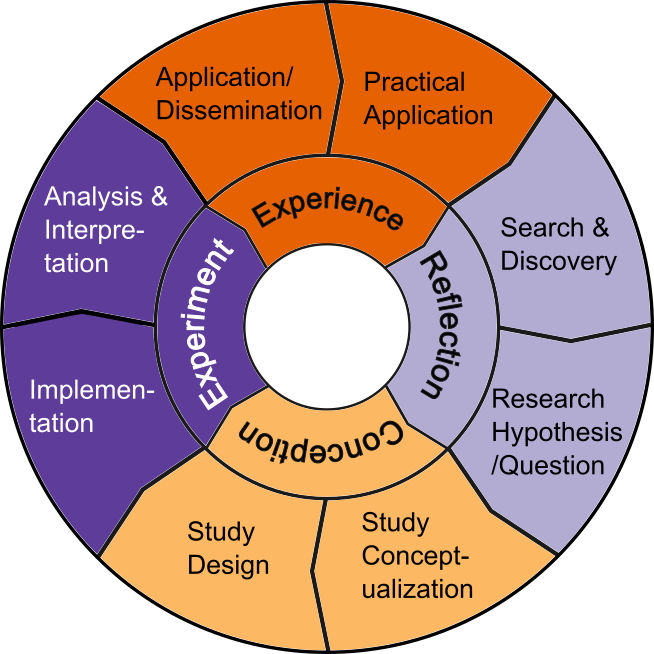
\includegraphics[width=0.7\linewidth,height=\textheight,keepaspectratio]{img/Research_cycle.png}

    }

    \caption{\label{fig-research_cycle}The research cycle based on
    \autocite{wildt2009forschendes} integrates the typical research
    process with the learning process.}

    \end{figure}%

    In the second example a GPT-like attention model is trained to
    classify data gained from the James-Webb telescope. Due to vast
    amounts of data and the continuous stream of new data research
    software engineering is needed to implement a pipeline for data
    cleaning, data warehousing and in-time analysis. In this case, the
    analysis \& interpretation phase (4) has much more relevance.
    Another point of this is example is that data science competencies
    such as vectorization of algorithms, statistical analysis, machine
    learning etc. are interconnected with competencies from software
    engineering such as software architectures, software project
    management, and database programming. In this case the distinction
    between DS competencies and RSE competencies is very fluid.

    The main argument behind these examples is that data science and
    research software engineering have a lot in common in terms of
    software development for science but show major differences where
    they are placed in the research process. This reframes the questions
    like ``how much programming is in DS'' or ``how much engineering is
    in RSE'' to a more structured approach of which cross-cutting
    functions exist in the research cycle that require computational
    means and which functions are part of the core identity of data
    scientists or research software engineers.

    As a working hypothesis based on the example above and experience in
    the field we assume the following: {[}H1{]} RSE focuses more on
    concept development (if the research is computationally heavy),
    design, implementation and dissemination, i.e.~phases 1,2,3,6
    whereas DS focuses more on analysis, interpretation and
    dissemination (phases 4,5,6). Moreover, a second hypothesis would be
    that RSE often plays a role in shaping the context of the research
    {[}H2a{]}, such as integrating projects with similar concerns, open
    source development and institutional needs. In contrast, data
    science is exclusively embedded in the research {[}H2b{]}.

    The focal point of the following chapter will revisiting existing
    ideas for DS and RSE curricula and map the competences outlined
    there to the phases in the research process. This should give the
    abstract discussion above empirical grounding and can be used to
    test the hypothesis.

    \section{Method}\label{method}

    In the following the contents of \autocite{GI2021DataScience} is
    parsed as the most current examples of data science curricula in the
    German research context. The contents are inspected for obvious
    links to the research process and interpreted if no explicit
    connections are made. Further sources for data science curriculum is
    the output of the Edison Project \autocite{EDSF2017} and the
    OpenDS4all Project \autocite{OpenDS4All2020}.

    For the RSE side the contents of \autocite{Goth2024RSE} are used as
    a basis as well as the current state of the RSE-Curriculums project
    \autocite{RSECurriculums2021}. For the RSE competencies the RSE
    community has developed short codes. These are attached in the
    glossary in the attached repository \autocite{ds2rse2025}.

    In addition, relevant competences from the research data management
    field \autocite{petersen_2025_15025246} are included as they
    intersect with both DS and RSE.

    In terms of methodology it should be noted that this approach
    follows a community-driven consensus building. It should not be
    mistaken for a review study with measurable intersubjectivity based
    on instruments like PRISMA \autocite{Page2021PRISMA}.

    The lists of extracted DS and RSE competency clusters can be found
    in \autocite{ds2rse2025}. We also plan to publish a full table of
    RSE competencies (and possible DS competencies) sorted by clusters.
    In terms of this top-level discussion the competency clusters are
    sufficient to compare the differences with regard to the research
    cycle.

    \section{Discussion}\label{discussion}

    H1 could not be confirmed in the strict sense. Although the compiled
    competency clusters show that there is a stronger focus on certain
    stages of the research process for both RSE and DS competencies,
    both can be interpreted more generally to encompass all stages of
    the research cycle. Moreover, there are some competency description
    that seem very similar such as the focus on the research cycle for
    RSE and the data science lifecycle for DS. In terms of methodology
    simply comparing the existing mentions of competencies should not be
    regarded as the best possible proxy to the actual distribution in
    the field. A survey study asking practitioners and researchers where
    in the process they would place DS and RSE would yield far more
    convincing results. Still, self-evaluation might also be biased
    depending on the identity of the people working the in the
    respective fields.

    \begin{figure}[h!]
    \centering
    \begin{minipage}{0.48\textwidth}
    \centering
    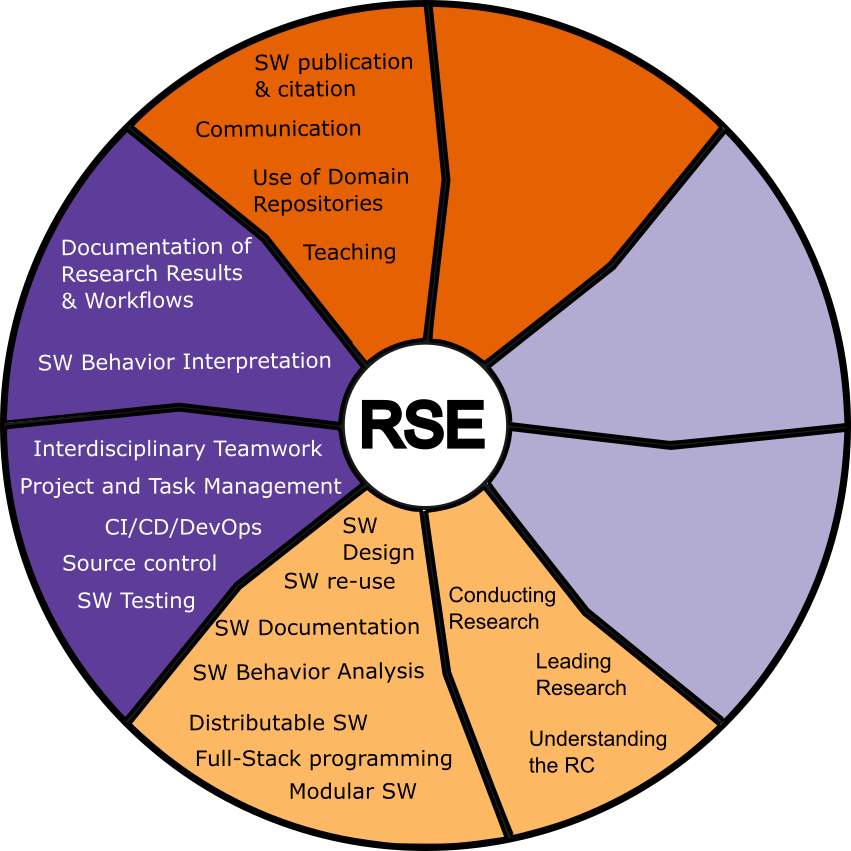
\includegraphics[width=\linewidth]{img/RC_RSE.png}
    \caption{RSE Competences in the Research Cycle}
    \label{fig:rc_rse}
    \end{minipage}\hfill
    \begin{minipage}{0.48\textwidth}
    \centering
    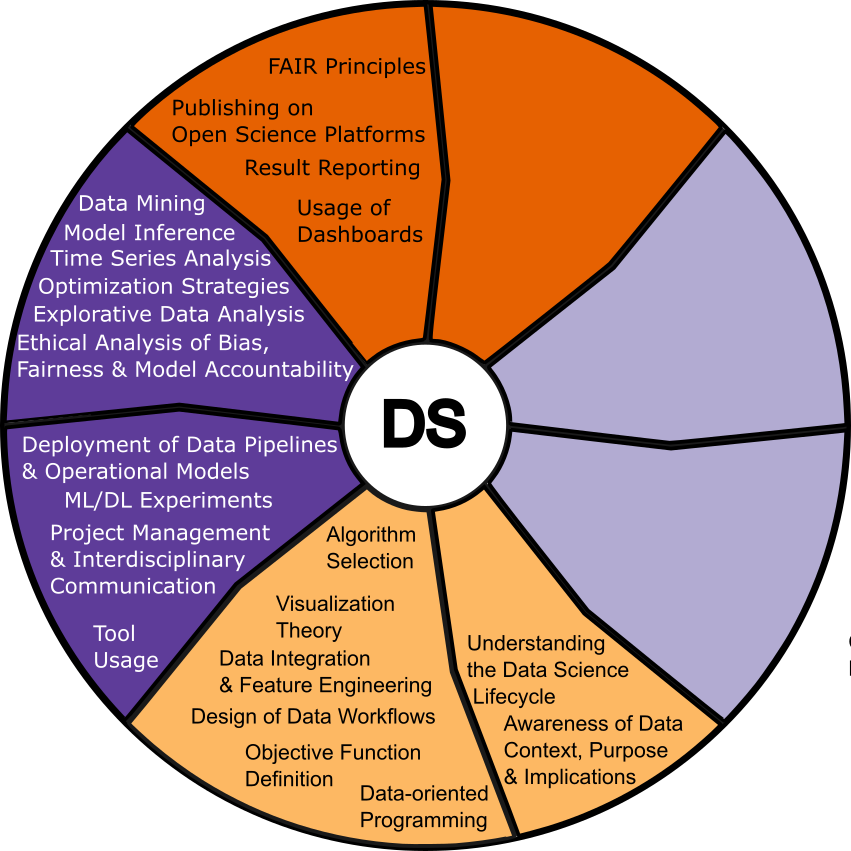
\includegraphics[width=\linewidth]{img/RC_DS.png}
    \caption{DS Competences in the Research Cycle}
    \label{fig:rc_ds}
    \end{minipage}
    \end{figure}

    The most clear differences between DS and RSE are found in the
    design stage and the analysis stage. The design stage holds most of
    the competency clusters the RSE community defined. The DS
    counterpart is very general and many competencies listed there could
    in fact be construed as RSE-competencies that are imported for more
    complex cases. In contrast, the analysis stage is more connected to
    DS. This can be explained by the historic challenges software
    development faces in terms of clear-cut evaluation but also by the
    distribution of labor: if the RSE-job ends with the developed
    software and the core experiment or study uses the software as a
    tool, the analysis part is then handed over to the respective field
    specialists.

    Another reason for the design focus of RSE is the limited resources
    available. It is very time-consuming to both evaluate the impact of
    technology and also to evaluate the technology itself and its impact
    on the study. Comprehensive methods like Directed Acyclic Graph
    Modellings (DAGs) or Instrumental Variables try to tackle these
    nested evaluation issues but have not found widespread use. For that
    reason, the evaluation often concludes with the evaluation of the
    design part with instruments like the Technology Acceptance Model
    (TAM) or usability scales.

    H2 also had to be rejected: in fact, DS seems to contain more
    aspects outside the research cycle than RSE. Even though the core
    analysis of data component is very embedded in research, DS has a
    lot of institutional, political and legal challenges. Research Data
    Management (RDM) could be named as the most prominent of these. Due
    to the strong overlap of non-research related competencies, a joint
    list competency clusters was compiled that lists the competences
    that are not research cycle related (also in the repository
    \autocite{ds2rse2025}).

    The long list of transversal competencies begs the question if there
    are also technical competences that overlap. Even though this was
    not the focus of the analysis, these can be easily spotted by
    investigating the shift of data analysis to artificial intelligence
    based methods. Training, fine-tuning and mainstreaming large
    language models requires more and more computing power, stable
    infrastructure and network components. On the other hand, CPU-based
    software-engineering becomes less demanding and also profits from
    AI-generated algorithm and code development. However, not all
    software engineering boils down to the current AI-hype. In summary,
    there is no clear way of generalizing whether DS or RSE need more
    and deeper understanding of computer science.

    \section{Conclusion}\label{conclusion}

    (planned/potential future work on this)

    \printbibliography

% Bibliography



\end{document}
